\chapter{Algorithme de résolution}
Un exemple de résolution pas à pas est donné dans l'annexe \ref{annexe_algo_action} en page \pageref{annexe_algo_action}.
\section{Description de l'algorithme}


L'algorithme de résolution est implémenté dans la classe \texttt{Ordi(Joueur)} du module \texttt{bn\_joueur.py}, dans la méthode \texttt{Ordi.coup\_suivant(self)}.\\
Il fonctionne en deux temps : dans un premier temps une phase de tir en aveugle et, une fois qu'une case a été touchée, une phase de tir ciblé jusqu'à ce que le bateau soit coulé.

L'attribut \texttt{Ordi.case\_courante} contient la case qui est entrain d'être jouée.
\subsection{Phase de tir en aveugle}
Lors de cette phase, l'algorithme va tirer sur la case qui peut contenir le plus de bateau comme vu au chapitre \ref{chap_grille}, section \ref{opti_aveugle} (page \pageref{opti_aveugle}). Cette phase est gérée par la méthode \texttt{Ordi.make\_case\_aleatoire(self)}.

C'est la méthode la plus efficace que nous ayons trouvée. Néanmoins nous avons fait d'autres essais avec d'autres méthodes mais celles-ci étaient beaucoup moins performantes, que ce soit en nombre de coups pour la résolution, qu'en temps :
\begin{itemize}
\item La première méthode consiste tout simplement à tirer au hasard sur une case vide.
\item On peut raffiner la méthode précédente en ne tirant que sur une case sur deux (le plus petit bateau étant de taille 2, chaque bateau tombe obligatoirement sur une case noire du damier).
\item Nous avons aussi essayé de déterminer la case la plus probable en créant un échantillon d'un certain nombre $n$ de répartitions aléatoires des bateaux restant sur le grille et en comptant, pour chaque case, le nombre de bateaux la contenant. Les performances en nombre d'essais étaient satisfaisantes, mais le temps de calcul beaucoup trop élevé. Voici un tableau récapitulatif de quelques essais avec différents paramètres :

\medskip

\begin{center}
\begin{tabular}{|l|c|c|c|c|}
\hline
Taille des échantillons & 100 & 1\,000 & 10\,000 & 100\,000\\
\hline
Nombre de parties & 10\,000 & 10\,000 & 1\,000 & 100\\
\hline
Nombre de coups moyens & 43,68 & 43,30 & 42,72 & 42,63\\
\hline
Temps moyen par partie (en secondes) & 0,38 & 3,6 & 36,2 & 380\\
\hline 
\end{tabular}\\
\vspace*{0.1cm}
\textit{Temps mesurés sur un processeur Intel Core i7 4800-MQ à 2,7 GHz}
\end{center}

\medskip

Au final, le temps de résolution étant linéaire en $n$ pour des gains de performances négligeables, cette approche a été abandonnée.

\item Enfin, une dernière approche consisterait à déterminer tous les arrangements de bateaux possibles sur la grille à chaque coup, de manière récursive. Cette approche semble optimale mais malheureusement, vu le nombre astronomique de configurations, cette approche est irréalisable que ce soit en temps de calcul qu'en utilisation mémoire. 

\end{itemize}  

Lors de cette phase on va également, avant chaque coup, éliminer les cases dans lesquelles le plus petit bateau restant à trouver ne rentre pas.

\subsection{Phase de tir ciblé}
Lors de cette phase, on va utiliser une file d'attente dans la liste \texttt{Ordi.queue} qui va contenir la liste des prochaines cases à viser. On va également garder la trace des cases touchées sur ce bateau dans la liste \texttt{Ordi.liste\_touches}, ainsi que la première case touchée dans \texttt{Ordi.case\_touchee}.
\subsubsection{Premier tir}
Lors du premier tir touché après la phase de tir en aveugle, l'attribut \texttt{Ordi.case\_touchee} reçoit la case courante qui sera également ajoutée à \texttt{Ordi.liste\_touches}. Puis on va remplir la file d'attente avec les cases adjacentes à la case touchée.

L'algorithme va également vérifier si le plus petit bateau ne peut pas rentrer dans une direction. Imaginons, par exemple, que le plus petit bateau restant soit de taille 3 et qu'on vienne de toucher la case $(3,0)$ dans la configuration suivante :

\begin{center}
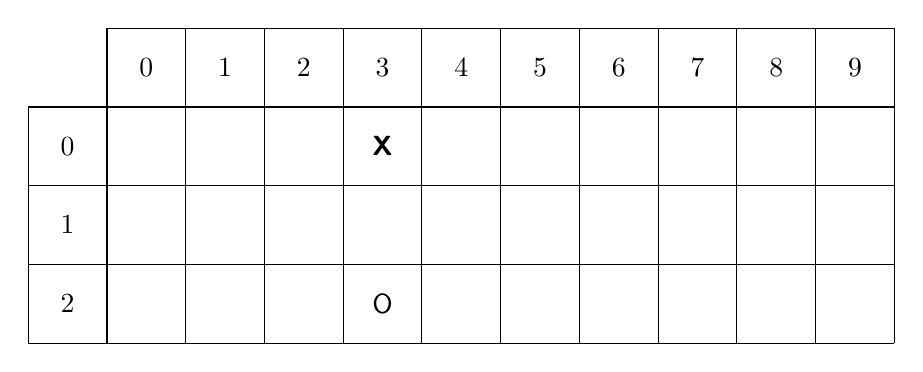
\begin{tikzpicture}
\draw (0,1)--(10,1);
\draw (-1,0)--(10,0);
\draw (-1,-1)--(10,-1);
\draw (-1,-2)--(10,-2);
\draw (-1,-3)--(10,-3);
\foreach \x in {0,1,...,10}{
\draw (\x,1)--(\x,-3);
}
\draw (-1,0)--(-1,-3);
\foreach \x in {0,1,...,9}{
\draw (\x+0.5,0.5) node{\x};
}
\draw (-0.5, -0.5) node{$0$};
\draw (-0.5, -1.5) node{$1$};
\draw (-0.5, -2.5) node{$2$};

\draw (3.5, -0.5) node{\textbf{\textsf{X}}};

\draw (3.5, -2.5) node{\textsf{O}};
\end{tikzpicture}\\
\textit{Le bateau de taille 3 ne rentre pas verticalement}
\end{center}
Il ne sert alors à rien de mettre la case $(3,1)$ dans la file d'attente car le plus petit bateau de taille 3 ne peut pas rentrer verticalement en $(3,0)$.

La construction de la liste des cases adjacentes possibles est effectuée par la méthode \texttt{Ordi.add\_adjacentes\_premiere(self)}.

\medskip

 Enfin, on va classer la file d'attente en ordre décroissant de nombre de bateaux possibles comme vu au chapitre \ref{chap_grille}, section \ref{opti_touche} (page \pageref{opti_touche}) avec la méthode \texttt{Ordi.shuffle\_queue(self)}.

\subsubsection{Deuxième tir}
Lors du deuxième tir (c'est à dire sur la première case de la file d'attente), on peut soit toucher, soit manquer.
\begin{itemize}
\item Si on touche alors, grâce à la méthode \texttt{Ordi.update\_queue\_touche(self)}, on détermine la direction du bateau (horizontal ou vertical) en comparant les coordonnées de \texttt{Ordi.case\_courante} et \texttt{Ordi.case\_touchee} et on enlève les cases de la file d'attente qui ne sont pas dans la bonne direction. On ajoute enfin la case à l'extrémité de la configuration créée à la file d'attente et on met à jour la liste \texttt{Ordi.liste\_touches}. 
\item Si on manque, alors on a peut-être bloqué une direction.\\
La méthode \texttt{Ordi.update\_queue\_manque(self)} se charge de cette vérification et élimine la case en face de la case jouée si besoin de la file d'attente.\\
Regardons un exemple. Imaginons que le plus petit bateau à trouver soit de taille 4 et que la première case touchée soit la case $(3,0)$. Nous venons de manquer la case $(4,0)$. Alors le bateau de taille 4 ne rentre plus horizontalement et on peut éliminer la case $(2,0)$ :

\begin{center}
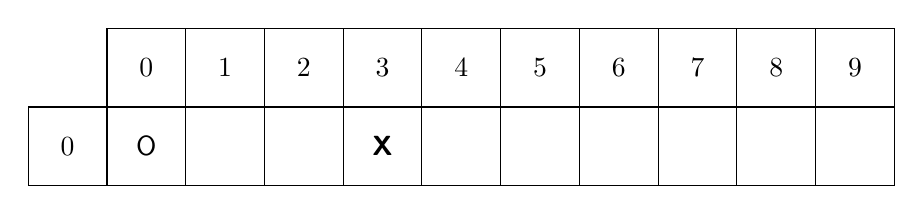
\begin{tikzpicture}
\draw (0,1)--(10,1);
\draw (-1,0)--(10,0);
\draw (-1,-1)--(10,-1);
\foreach \x in {0,1,...,10}{
\draw (\x,1)--(\x,-1);
}
\draw (-1,0)--(-1,-1);
\foreach \x in {0,1,...,9}{
\draw (\x+0.5,0.5) node{\x};
}
\draw (-0.5, -0.5) node{$0$};

\draw (3.5, -0.5) node{\textbf{\textsf{X}}};

%\draw (5.5, -0.5) node{\textsf{O}};
\draw (0.5, -0.5) node{\textsf{O}};
\end{tikzpicture}\\
\textit{À ce niveau, le bateau de taille 4 rentre horizontalement.}
\end{center}
\medskip
\begin{center}
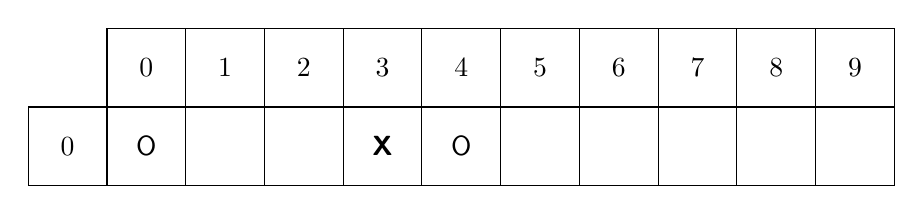
\begin{tikzpicture}
\draw (0,1)--(10,1);
\draw (-1,0)--(10,0);
\draw (-1,-1)--(10,-1);
\foreach \x in {0,1,...,10}{
\draw (\x,1)--(\x,-1);
}
\draw (-1,0)--(-1,-1);
\foreach \x in {0,1,...,9}{
\draw (\x+0.5,0.5) node{\x};
}
\draw (-0.5, -0.5) node{$0$};

\draw (3.5, -0.5) node{\textbf{\textsf{X}}};

%\draw (5.5, -0.5) node{\textsf{O}};
\draw (4.5, -0.5) node{\textsf{O}};
\draw (0.5, -0.5) node{\textsf{O}};
\end{tikzpicture}\\
\textit{Après ce coup, le bateau de taille 4 ne rentre plus horizontalement et on peut éliminer la case $(2,0)$.}
\end{center}
Pour ce faire, on détermine la direction dans laquelle on vient de tirer en comparant les coordonnées de \texttt{Ordi.case\_courante} et \texttt{Ordi.case\_touchee} et on regarde si le plus petit bateau rentre dans la direction en face.

\end{itemize}   

\subsubsection{Tirs suivants}
Une fois que la direction du bateau est déterminée, à chaque fois qu'on touche une case, on ajoute à la file d'attente sa case adjacente dans la bonne direction.

Enfin on s'arrête lorsque la file d'attente est vide (on a manqué les deux extrémités) ou lorsque la taille du bateau touché est égale à la plus grande taille du bateau sur la grille avec \texttt{Ordi.test\_plus\_grand(self)} et, dans ce cas, on vide la file d'attente. 
%La méthode \texttt{Ordi.liste\_touches} permet de garder la trace des cases touchées sur ce bateau et d'en déterminer le nombre de cases.

Au prochain tour, on sait qu'un bateau vient d'être coulé lorsque la file d'attente est vide et \texttt{Ordi.liste\_touches} ne l'est pas. Dans ce cas on marque ses cases adjacentes comme impossibles et on l'enlève de la liste des bateaux à chercher. On n'a plus alors qu'à repartir dans une phase de tir en aveugle.
\newpage
\subsection{Algorithme complet}
Voici l'algorithme complet de la résolution :

\begin{algo1}
La file d'attente est une liste vide\\
liste\_touches est une liste vide\\
Tant que le grille n'est pas résolue :\\
\tab{1}Si la file d'attente est vide :\\
\tab{2}Si liste\_touches n'est pas vide :\\
\tab{3}On enlève le bateau de taille len(liste\_touches)\\
\tab{3}On élimine les cases adjacentes à celles de liste\_touches\\
\tab{3}On vide liste\_touches\\
\tab{2}On élimine les zones trop petites\\
\tab{2}case\_courante reçoit une case en aveugle\\
\tab{1}Sinon :\\
\tab{2}case\_courante reçoit le premier élément de la file d'attente\\
\tab{2}On enlève cette case de la file d'attente\\
\tab{1}On tire sur case\_courante\\
\tab{1}Si on a touché :\\
\tab{2}Si liste\_touches est vide :\\
\tab{3}On ajoute case\_courante dans liste\_touches\\
\tab{3}case\_touchee\sto case\_courante\\
\tab{3}On ajoute ses cases adjacentes dans la file d'attente\\
\tab{4}(en testant également les directions impossibles éventuelles)\\
\tab{2}Sinon :\\
\tab{3}Si len(liste\_touches) == 1 :\\
\tab{4}On détecte la direction du bateau\\
\tab{3}On met à jour la file d'attente\\
\tab{4}(avec la case adjacente à case\_courante dans la bonne direction)\\
\tab{2}Si le bateau touché est le plus grand restant :\\
\tab{3}On vide la file d'attente\\
\tab{1}Sinon :\\
\tab{2}Si len(liste\_touches) == 1 :\\
\tab{3}On met à jour la file d'attente\\
\tab{4}(on élimine éventuellement la case en face de case\_touchee)\\
On affiche le nombre de coups\\
\end{algo1}

\newpage

\section{Étude statistique}
Le module \texttt{bn\_stats.py} fournit, dans la classe \texttt{Stats}, les outils pour analyser statistiquement une distribution de valeurs (calculs des indicateurs statistiques classiques, représentation en histogramme et diagramme en boîte grâce aux modules \texttt{numpy} et \texttt{matplotlib}).\\
Un test de l'algorithme de résolution sur $n=1\,000\,000$ parties donne les résultats suivants :

\begin{center}\label{histo_algo}
\fbox{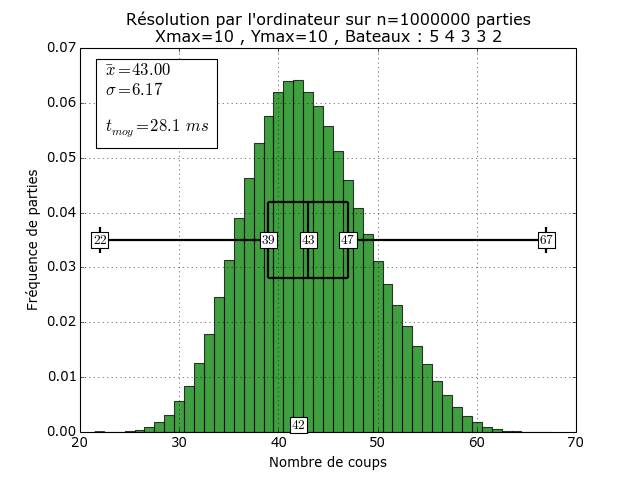
\includegraphics[scale=0.7]{./media/distrib_1000000.png}}
\end{center}

Notons les excellentes performances avec une moyenne de 42,06 coups pour un temps de résolution moyen de seulement 31,2 ms\footnote{Temps mesuré sur un processeur Intel Core i7 4800-MQ à 2,7 Ghz} par partie.

La liste des données obtenues est donnée en annexe \ref{annexe_stats} page \pageref{annexe_stats}.

%La forme de cette distribution semble correspondre à une loi normale asymétrique. Ce résultat sera développé en annexe \ref{annexe_stats} page \pageref{annexe_stats}.